\documentclass[compress]{beamer}
\usepackage[brazil]{babel}
\usepackage{amsmath}
\usepackage{graphicx}
\usepackage{listings}

%%%%%%%%%%%%%%%%%%%%%%%%%%%%%
% C O N F I G U R A Ç Õ E S %
%%%%%%%%%%%%%%%%%%%%%%%%%%%%%
\definecolor{listinggray}{gray}{0.9}
\definecolor{lbcolor}{rgb}{1,1,1}

\lstset{
	backgroundcolor=\color{lbcolor},
	tabsize=4,
	rulecolor=,
	language=matlab,
    basicstyle=\scriptsize,
    upquote=true,
    aboveskip={1.5\baselineskip},
    columns=fixed,
    showstringspaces=false,
    extendedchars=true,
    breaklines=true,
    prebreak = \raisebox{0ex}[0ex][0ex]{\ensuremath{\hookleftarrow}},
    frame=single,
    showtabs=false,
    showspaces=false,
    showstringspaces=false,
    identifierstyle=\ttfamily,
}

\renewcommand{\lstlistingname}{Código}
\renewcommand{\lstlistlistingname}{Lista de Códigos}

\usetheme{Ilmenau}
%vinho
%\usecolortheme[RGB={75,11,31}]{structure}
%verde
%\usecolortheme[RGB={35,75,11}]{structure}
%azul
\usecolortheme[RGB={12,67,102}]{structure}
\setbeamercovered{transparent}
\setbeamertemplate{blocks}[rounded][shadow=true]
\setlength{\tabcolsep}{1mm}
%\setbeamertemplate{footline}[frame number]
\setbeamertemplate{navigation symbols}{}
\setbeamertemplate{headline}[default]
\setbeamertemplate{footline}[default]
\setbeamertemplate{footline}{\hspace*{.5cm}\scriptsize{\hfill\vspace*{0.3cm}\insertframenumber\hspace*{.5cm}}}

\newenvironment{changemargin}[2]{%
  \begin{list}{}{%
    \setlength{\topsep}{0pt}%
    \setlength{\leftmargin}{#1}%
    \setlength{\rightmargin}{#2}%
    \setlength{\listparindent}{\parindent}%
    \setlength{\itemindent}{\parindent}%
    \setlength{\parsep}{\parskip}%
  }%
  \item[]}{\end{list}}

%%%%%%%%%%%
% C A P A %
%%%%%%%%%%%

\title{Classificação de \textit{issues} do Github relacionadas a Segurança}

\subtitle{Aprendizagem de Máquina}

\author{Bruno Gonçalves de Oliveira \\
       {\footnotesize\ttfamily bruno.mphx2@gmail.com} \\
       Diogo Cezar Teixeira Batista \\
       {\footnotesize\ttfamily diogocezar@utfpr.br}
}

\institute{\large Universidade Federal do Paraná - UFPR}

\date{Curitiba - 2020}

\begin{document}

%%%%%%%%%%%%%%%%%%%%%%%%%%%%%%%%
% S L I D E S  I N I C I A I S %
%%%%%%%%%%%%%%%%%%%%%%%%%%%%%%%%

\begin{frame}
  \titlepage
\end{frame}
\begin{frame}
  \frametitle{Agenda}
  \tableofcontents
\end{frame}

%%%%%%%%%%%%%%%%%%%%%
% C A P Í T U L O S %
%%%%%%%%%%%%%%%%%%%%%

\section[Introdução]{Introdução}

\begin{frame}
  \frametitle{Introdução}
  \begin{itemize}
    \item Gerenciamento e manutenção de arquivos: desafio;
          \begin{itemize}
            \item backups não realizados;
            \item sobrescrita de arquivos;
            \item difícil manutenabilidade em times;
          \end{itemize}
    \item Diferentes soluções no mercado: \textit{CVS}, \textit{Subversion}, \textit{TFS}, \textit{Mercurial}.
  \end{itemize}
\end{frame}

\begin{frame}
  \frametitle{GitHub}
  \begin{itemize}
    \item \textit{Git} + \textit{GitHub} = \textit{OpenSource}.
    \item \textit{GitHub} que é uma plataforma para versionamento, gerenciamento e colaboração de projetos, que utiliza o \textit{Git} como base. \cite{Scott:ProGit}
  \end{itemize}
\end{frame}

\begin{frame}
  \frametitle{Controle de Issues}
  \begin{itemize}
    \item Dentre outras ferramentas temos o controle de \textit{Issues:}.
          \begin{itemize}
            \item documentar possíveis \textit{bugs}, melhorias, ou novas \textit{features} para os projetos
          \end{itemize}
  \end{itemize}
\end{frame}

\begin{frame}
  \frametitle{Exemplo Issues}
  \begin{figure}[htbp]
    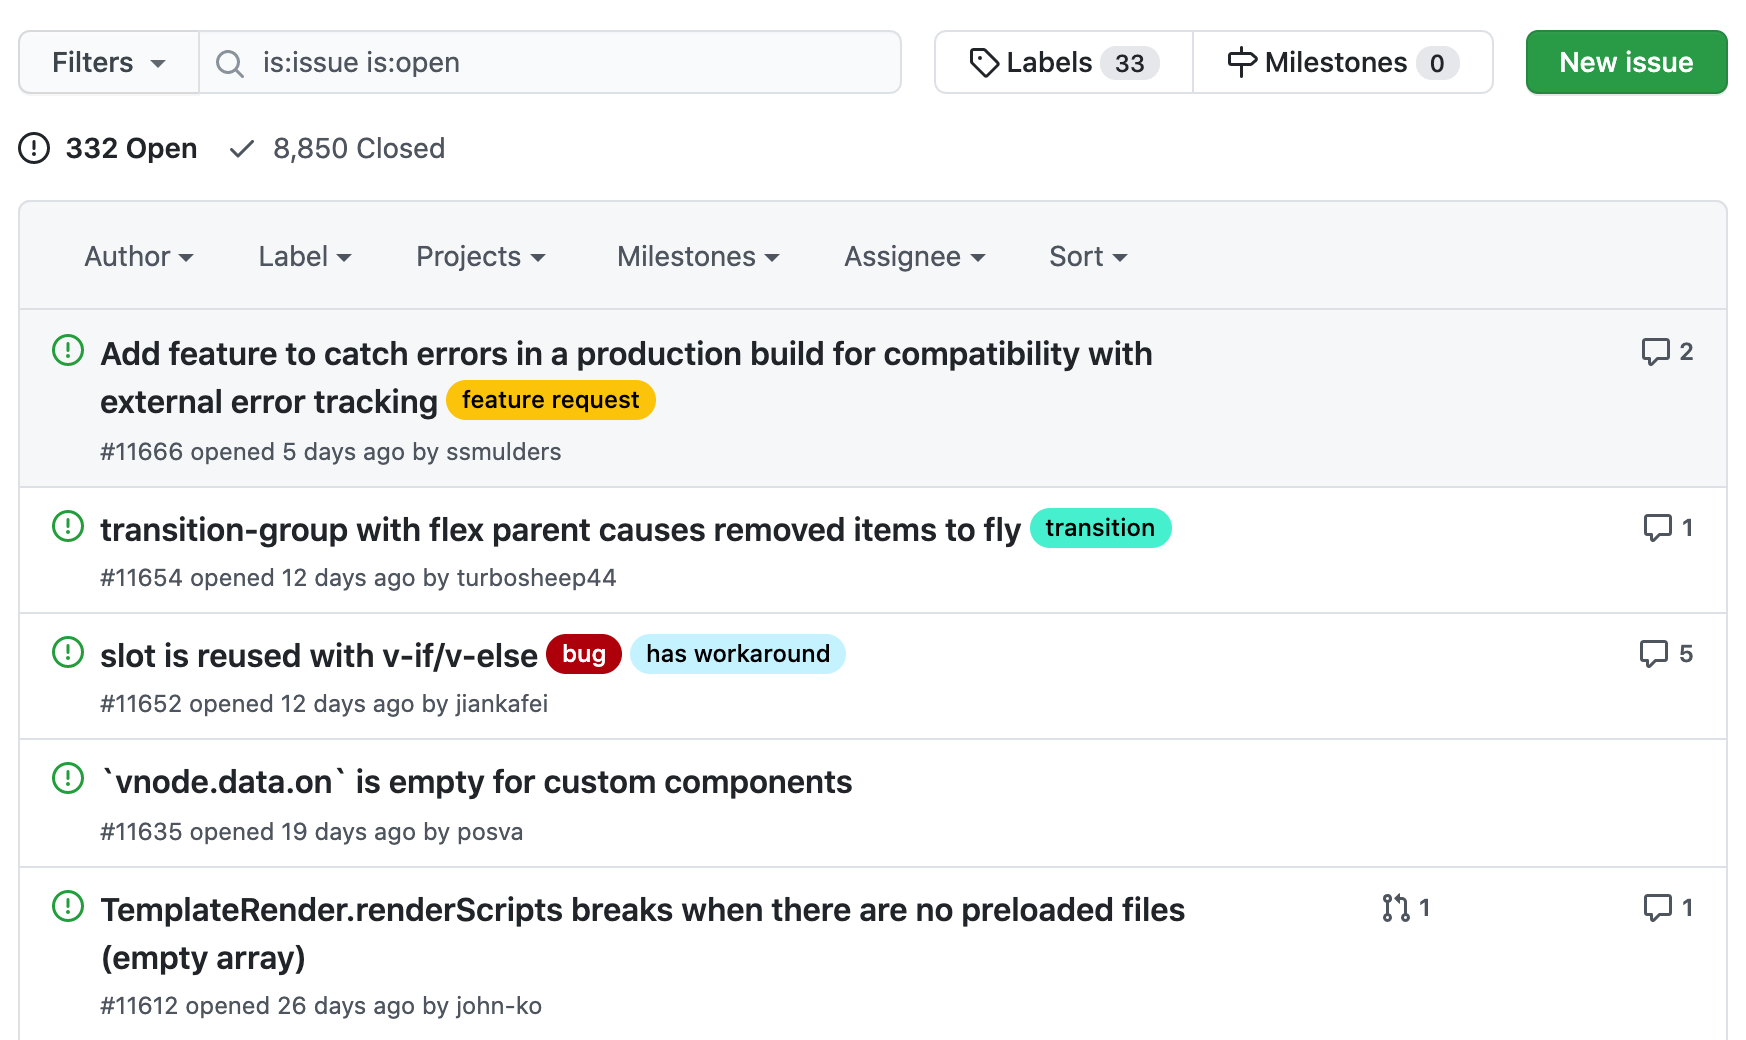
\includegraphics[width=\textwidth]{images/issues_example.png}
    \caption{Exemplos de Issues do Projeto Vue.js}
  \end{figure}
\end{frame}

\begin{frame}
  \frametitle{Issues sobre Segurança}
  \begin{itemize}
    \item Eventualmente, as \textit{issues} podem estar relacionadas a tópicos de segurança.
    \item Quando consideradas críticas, podem ser analisadas por outros especialistas;
    \item Como identificar quais \textit{issues} que são relacionadas com segurança?
    \item Como classificar estas \textit{issues} para que especialistas possam analisar os cógidos?
  \end{itemize}
\end{frame}

\begin{frame}
  \frametitle{Proposta do Trabalho}
  \begin{itemize}
    \item Criação de uma ferramenta que utilize técnicas de \textbf{aprendizagem de máquina} para o desenvolvimento de um classificador que consiga analisar as palavras contidas nas mensagens das \textit{issues} de um dado projeto, e classificar se esta \textit{issue} está ou não relacionada no contexto de segurança da informação.
  \end{itemize}
\end{frame}
\section[Obtenção dos Dados]{Obtenção dos Dados}

\begin{frame}[fragile]
  \frametitle{Obtenção dos Dados}
  \begin{itemize}
    \item Utilizou-se o \textit{github-csv-tools\footnote{https://github.com/gavinr/github-csv-tools}} que possibilita a exportação dos dados de um repositório do \textit{GitHub}, salvando as informações em um arquivo no formato CSV.
    \item Dados tratados para um CSV com 2 colunas:
  \end{itemize}
  \begin{lstlisting}[caption={CSV Exemplo com Base de Dados},captionpos=b,frame=single,label={code:csv_example}]
    security,PushObserver can be used to push serverinitiated HTTP/2 requests into an OkResponseCache...
    not,Handle LOCKED in conversions.Motivation...
    \end{lstlisting}
\end{frame}

\begin{frame}
  \frametitle{Fonte de Dados}
  \begin{itemize}
    \item Base de Testes: \textit{issues} do projeto \textit{Wildfly\footnote{https://github.com/wildfly/wildfly}};
    \item Base de Treinamento: \textit{issues} dos projetos: \textit{okhttp\footnote{https://github.com/square/okhttp}}, \textit{jgit\footnote{https://github.com/eclipse/jgit}} e \textit{couchbase\footnote{https://github.com/couchbase}}
    \item Os dados de treinamento possuem \textbf{199} entradas, enquanto que para a base de teste foram utilizadas \textbf{211} entradas.
  \end{itemize}
\end{frame}
\section[Pré-processamento]{Pré-processamento}

\begin{frame}
  \frametitle{Pré-processamento}
  \begin{itemize}
    \item Completar...
  \end{itemize}
\end{frame}
\section[Extração de Características]{Extração de Características}

\begin{frame}[fragile]
  \frametitle{Extração de Características}
  \begin{itemize}
    \item Foram aplicadas as técnicas:
          \begin{itemize}
            \item Bag-of-Words;
            \item TF-IDF (term frequency-inverce document frequency);
          \end{itemize}
    \item Palavras mais relevantes: ['security', 'secure', 'vulnerable', 'leak', 'exception', 'crash', 'malicious',
          'sensitive', 'user', 'authentication', 'protect', 'vulnerability', 'authenticator', 'auth', 'npe']
  \end{itemize}
\end{frame}
\section[Resultados]{Resultados}

\begin{frame}
  \frametitle{Resultados}
  \begin{itemize}
    \item Completar...
  \end{itemize}
\end{frame}
\section[Conclusão]{Conclusão}

\begin{frame}
  \frametitle{Conclusão}
  \begin{itemize}
    \item Completar...
  \end{itemize}
\end{frame}

\begin{frame}
  \frametitle{Trabalhos Futuros}
  \begin{itemize}
    \item Completar...
  \end{itemize}
\end{frame}

%%%%%%%%%%%%%%%%%%%%%%%%%%%%%%
% S L I D E S    F I N A I S %
%%%%%%%%%%%%%%%%%%%%%%%%%%%%%%

\begin{frame}[allowframebreaks]
  \frametitle{References}
  \bibliographystyle{amsalpha}
  \bibliography{../report/IEEEexample.bib}
\end{frame}

\end{document}